\setcounter{step}{0}

\subsection{ Basic polievka }

\begin{ingredient}
  
      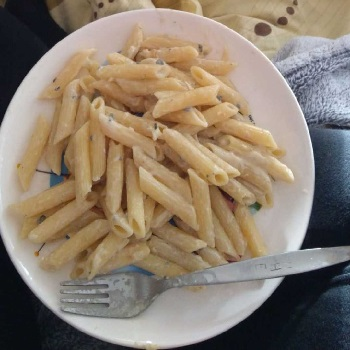
\includegraphics[height=5.5cm]{images/cestoviny}
  
  \def\portions{  }
  \textbf{ {\normalsize Ingrediencie (4porcie):} }

  \begin{main}
      \item 4 cà.S de sucre en poudre
      \item 1 cà.S de crème liquide
      \item 1 cà.S de miel
      \item 1 grosse noix de beurre
  \end{main}
  
    \begin{subingredient}{poleva}
        \item kŕdeľ ďatľov učí koňa žrať kôru
        \item nieco iné
    \end{subingredient}
  
    \begin{subingredient}{dalsia vec}
        \item aaa
        \item bb
    \end{subingredient}
  
\end{ingredient}
\begin{recipe}
\textbf{ {\normalsize Príprava:} }
\begin{enumerate}

  \item{urobime nieco}
  \item{potom nieco ine}
  \item{a este daco}
  \item{tato vec ma viac krokov: }
      \begin{enumerate}
          \item{lebo urobime toto}
          \item{a toto}\end{enumerate}
  \item{tato vec ma TIEZ viac krokov: }
      \begin{enumerate}
          \item{lebo urobime toto}
          \item{a toto}\end{enumerate}
  \item{a tiez toto}

\end{enumerate}
\end{recipe}

\begin{notes}
  Bla bla, nieco, poznamka
\end{notes}	
\clearpage
